\section{Durchführung}
\label{sec:Durchführung}

Der Versuchsaufbau ist in Abbildung \ref{fig:aufbau} zu sehen. Zunächst wird der Abstand $L$
vom Beugungsspalt zur Detektorblende gemessen. Der Detektor ist hier ein Photoelement.
Dieses misst elektromagnetische Wellen und erzeugt einen Strom, der dann gemessen wird.
Durch die Wärme im Photoelement entstehen freie Ladungsträger, die einen Strom erzeugen,
ohne dass elektromagnetische Wellen den Detektor erreichen. Nach Ausschalten des Lasers
wird dieser sogenannte Dunkelstrom $I_\text{dunkel}$ vor jeder Messreihe abgelesen.
Danach wird der Laser wieder eingeschaltet. Zur Messung der Lichtintensität wird der
angezeigte Strom $I$ notiert.

\begin{figure}
  \centering
  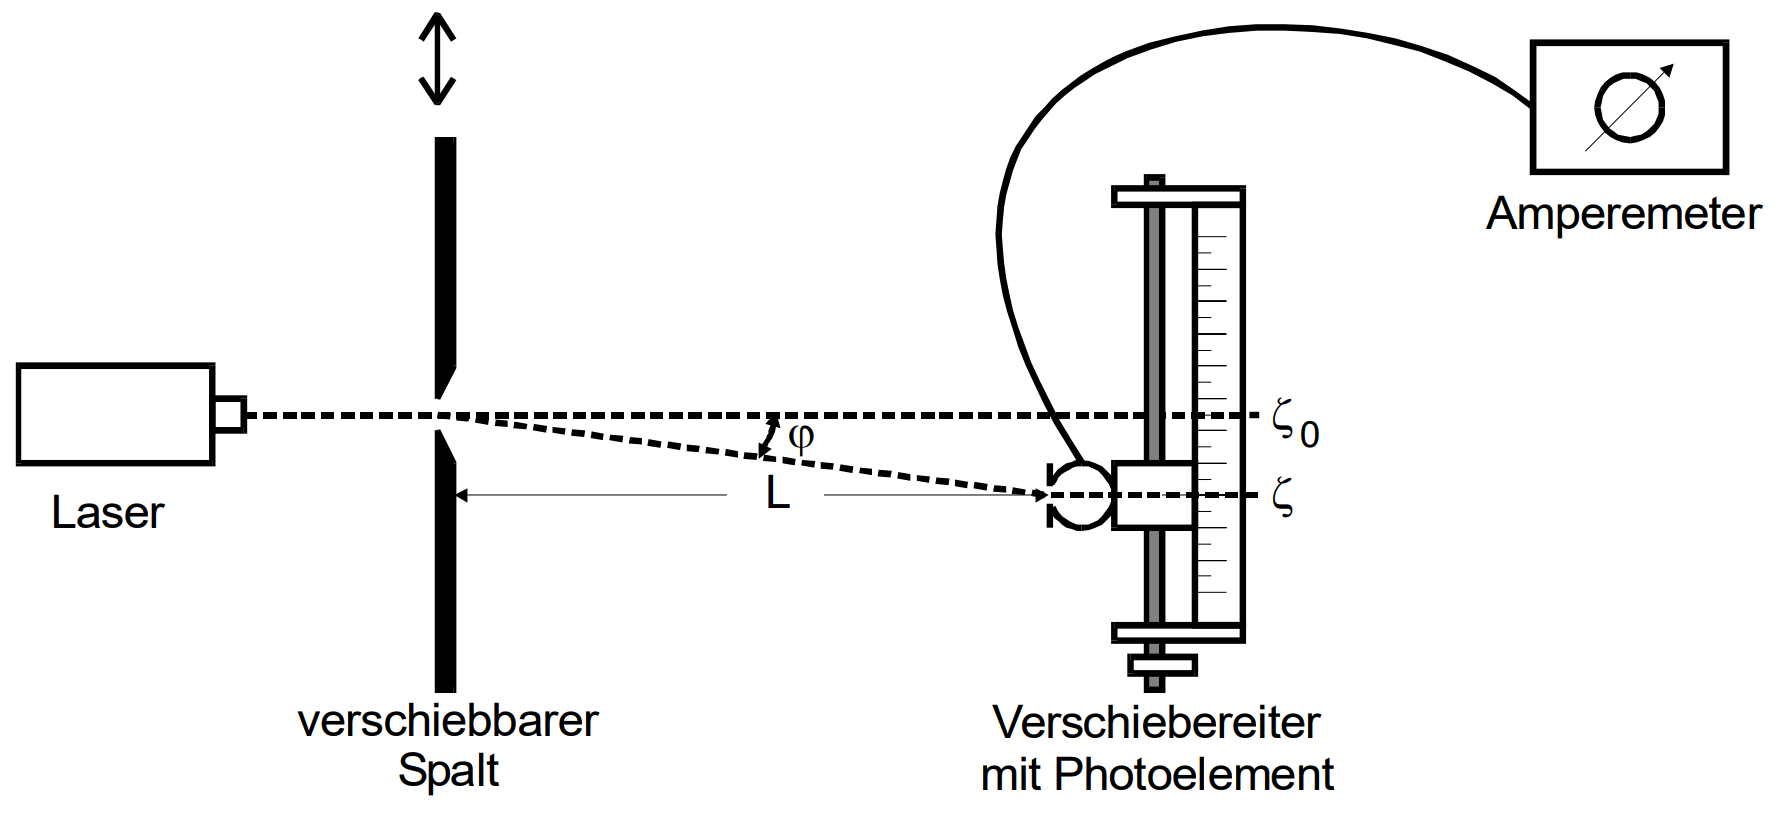
\includegraphics[width=260pt]{data/aufbau.png}
  \caption{Skizze der Versuchsanordnung \cite{Versuchsanleitung}}
  \label{fig:aufbau}
\end{figure}

Es werden die Beugungsbilder von zwei verschiedenen Einfachspalten und einem Doppelspalt
gemessen. Dafür wird der Dektor in der Beugungsebene orthogonal zum Lichteinfall
bewegt und der Strom $I$ gemessen. Je nach Bedarf werden die Intervalle, in denen der
Detektor bewegt wird, kleiner oder größer gewählt. Bei den beiden Einzelspalten
werden an den Rändern alle $\SI{0.5}{\milli\meter}$ und um das Hauptmaximum herum alle
$\SI{0.25}{\milli\meter}$ Messwerte aufgenommen. Beim Doppelspalt werden an den Rändern
alle $\SI{0.25}{\milli\meter}$ und in der Nähe des Hauptmaximums, sobald sehr starke
Änderungen der Intensität festzustellen sind, alle $\SI{0.125}{\milli\meter}$
Messwerte aufgenommen.
